\documentclass{article}

\usepackage[utf8]{inputenc}
\usepackage[english]{babel}
\usepackage{hyperref}
\usepackage{amsmath}
\usepackage{float}
\usepackage{cite}
\usepackage{url}
\usepackage{listings}
\usepackage{graphicx}
%\usepackage{parskip}
\usepackage{color}
\usepackage{tabularx}
\usepackage{booktabs}
\usepackage{titlesec}
\usepackage{geometry}
\usepackage[T1]{fontenc}

\newgeometry{vmargin={20mm}, hmargin={35mm,35mm}}

% https://tex.stackexchange.com/questions/60209/how-to-add-an-extra-level-of-sections-with-headings-below-subsubsection
\setcounter{secnumdepth}{4}

\titleformat{\paragraph}
{\normalfont\normalsize\bfseries}{\theparagraph}{1em}{}
\titlespacing*{\paragraph}
{0pt}{3.25ex plus 1ex minus .2ex}{1.5ex plus .2ex}

\definecolor{codegreen}{rgb}{0,0.6,0}
\definecolor{codegray}{rgb}{0.5,0.5,0.5}
\definecolor{codepurple}{rgb}{0.58,0,0.82}
\definecolor{backcolour}{rgb}{0.95,0.95,0.92}
\definecolor{lightgray}{rgb}{.9,.9,.9}
\definecolor{darkgray}{rgb}{.4,.4,.4}
\definecolor{purple}{rgb}{0.65, 0.12, 0.82}

\graphicspath{ {../assets/} }

\bibliographystyle{unsrt}

\lstdefinelanguage{JavaScript}{
    keywords={break, case, catch, continue, debugger, default, delete, do, else, false, finally, for, function, if, in, instanceof, new, null, return, switch, this, throw, true, try, typeof, var, void, while, with},
    morecomment=[l]{//},
    morecomment=[s]{/*}{*/},
    morestring=[b]',
    morestring=[b]",
    ndkeywords={class, export, boolean, throw, implements, import, this},
    keywordstyle=\color{blue}\bfseries,
    ndkeywordstyle=\color{darkgray}\bfseries,
    identifierstyle=\color{black},
    commentstyle=\color{purple}\ttfamily,
    stringstyle=\color{red}\ttfamily,
    sensitive=true
}
\lstdefinestyle{default}{
    backgroundcolor=\color{backcolour},
    commentstyle=\color{codegreen},
    keywordstyle=\color{magenta},
    numberstyle=\tiny\color{codegray},
    stringstyle=\color{codepurple},
    basicstyle=\ttfamily\footnotesize,
    breakatwhitespace=false,
    breaklines=true,
    captionpos=b,
    keepspaces=true,
    numbers=left,
    numbersep=5pt,
    showspaces=false,
    showstringspaces=false,
    showtabs=false,
    tabsize=2
}
\lstset{
    language=JavaScript,
    backgroundcolor=\color{lightgray},
    extendedchars=true,
    basicstyle=\footnotesize\ttfamily,
    showstringspaces=false,
    showspaces=false,
    tabsize=2,
    breaklines=true,
    showtabs=false,
    captionpos=b
}


\title{
    Decibel Threshold Event Displayer\\
    ~\\
    \small
    \textbf{Analyze Audio Files and detect Noise Pollution}
}
\author{
    Dominic Gernert (gernd1) \\
    Darius Degel (deged2) \\
    Lukas von Allmen (vonal3)
}
\date{\today}

\begin{document}
    \maketitle

\begin{table}[H]
    \centering
    \begin{tabularx}{\textwidth}{l X}
        \toprule
        School           & \textbf{Bern University of Applied Sciences} \\
        \midrule
        Module           & \textbf{BTI3031 - Project 1 (24/25)} \\
        \midrule
        Tutor            & \textbf{Dr. Simon Kramer} \\
        \bottomrule
    \end{tabularx}
    \label{tab:title-page}
\end{table}

\pagebreak
    \begin{abstract}\label{sec:abstract}

Noise pollution affects one in seven people in Switzerland, 
primarily caused by road traffic, railways, and air traffic, along with secondary sources such as construction sites and nightclubs. 
To address this issue, affected individuals must provide evidence, typically through audio recordings.
This project aims to create a free, open-source, and platform-independent application, which helps individuals in documenting noise pollution. \\
\\
The application processes *.WAV files, filters the data by a given threshold and
generates a PDF with an according plot which can be used as evidence.
For a meaningful interpretation of a *.WAV file, the user must provide a minimal and maximal dB(A) provided by an external tool,
such as smartphone apps like DecibelX. \\

\begin{table}[H]
    \centering
    \begin{tabularx}{\textwidth}{l X}
        \toprule
        License           & \textbf{\href{https://www.gnu.org/licenses/gpl-3.0.en.html}{GPL-3.0 licence (FLOSS)}} \\
        \midrule
        Application       & \textbf{\href{https://decibel-threshold-event-displayer.github.io/\#/}{dB threshold event displayer}} \\
        \midrule
        About Page        & \textbf{\href{https://decibel-threshold-event-displayer.github.io/\#/about}{About Decibel Threshold Event Displayer}} \\
        \midrule
        Repository        & \textbf{\href{https://github.com/decibel-threshold-event-displayer/decibel-threshold-event-displayer.github.io}{GitHub}} \\
        \bottomrule
    \end{tabularx}
    \label{tab:abstract-infos}
\end{table}

\-
%~\\

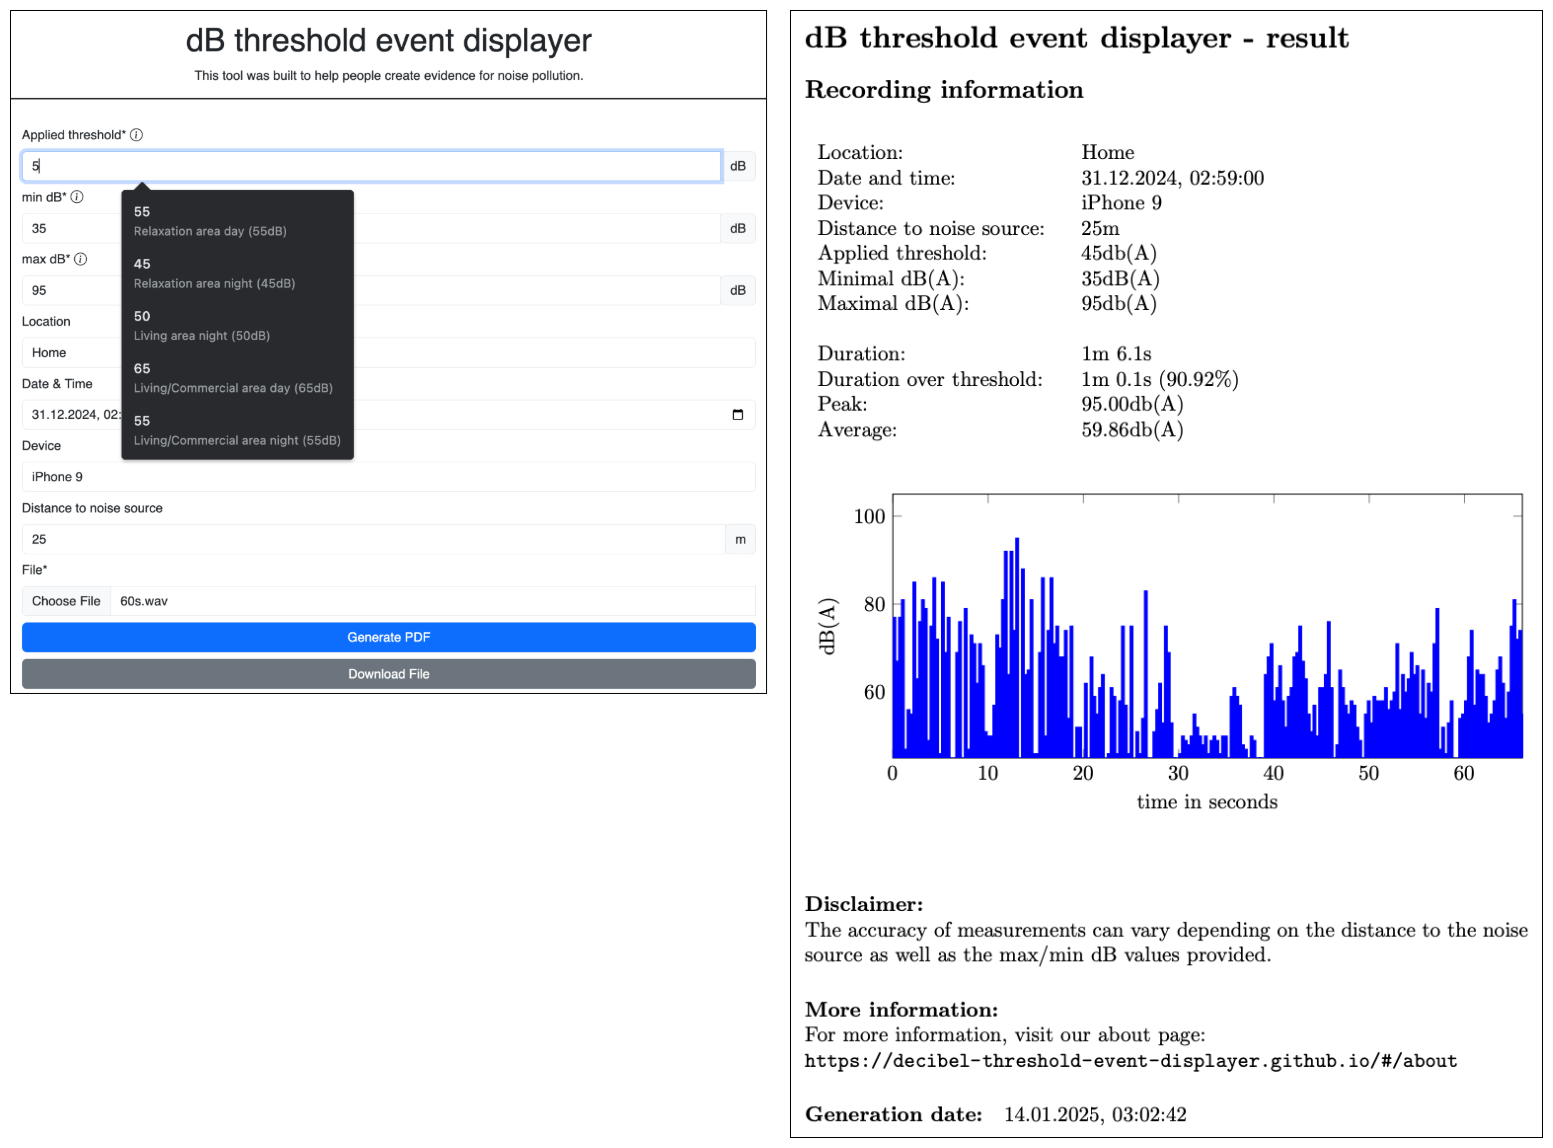
\includegraphics[width=0.8\textwidth]{../assets/abstract_preview.png}

%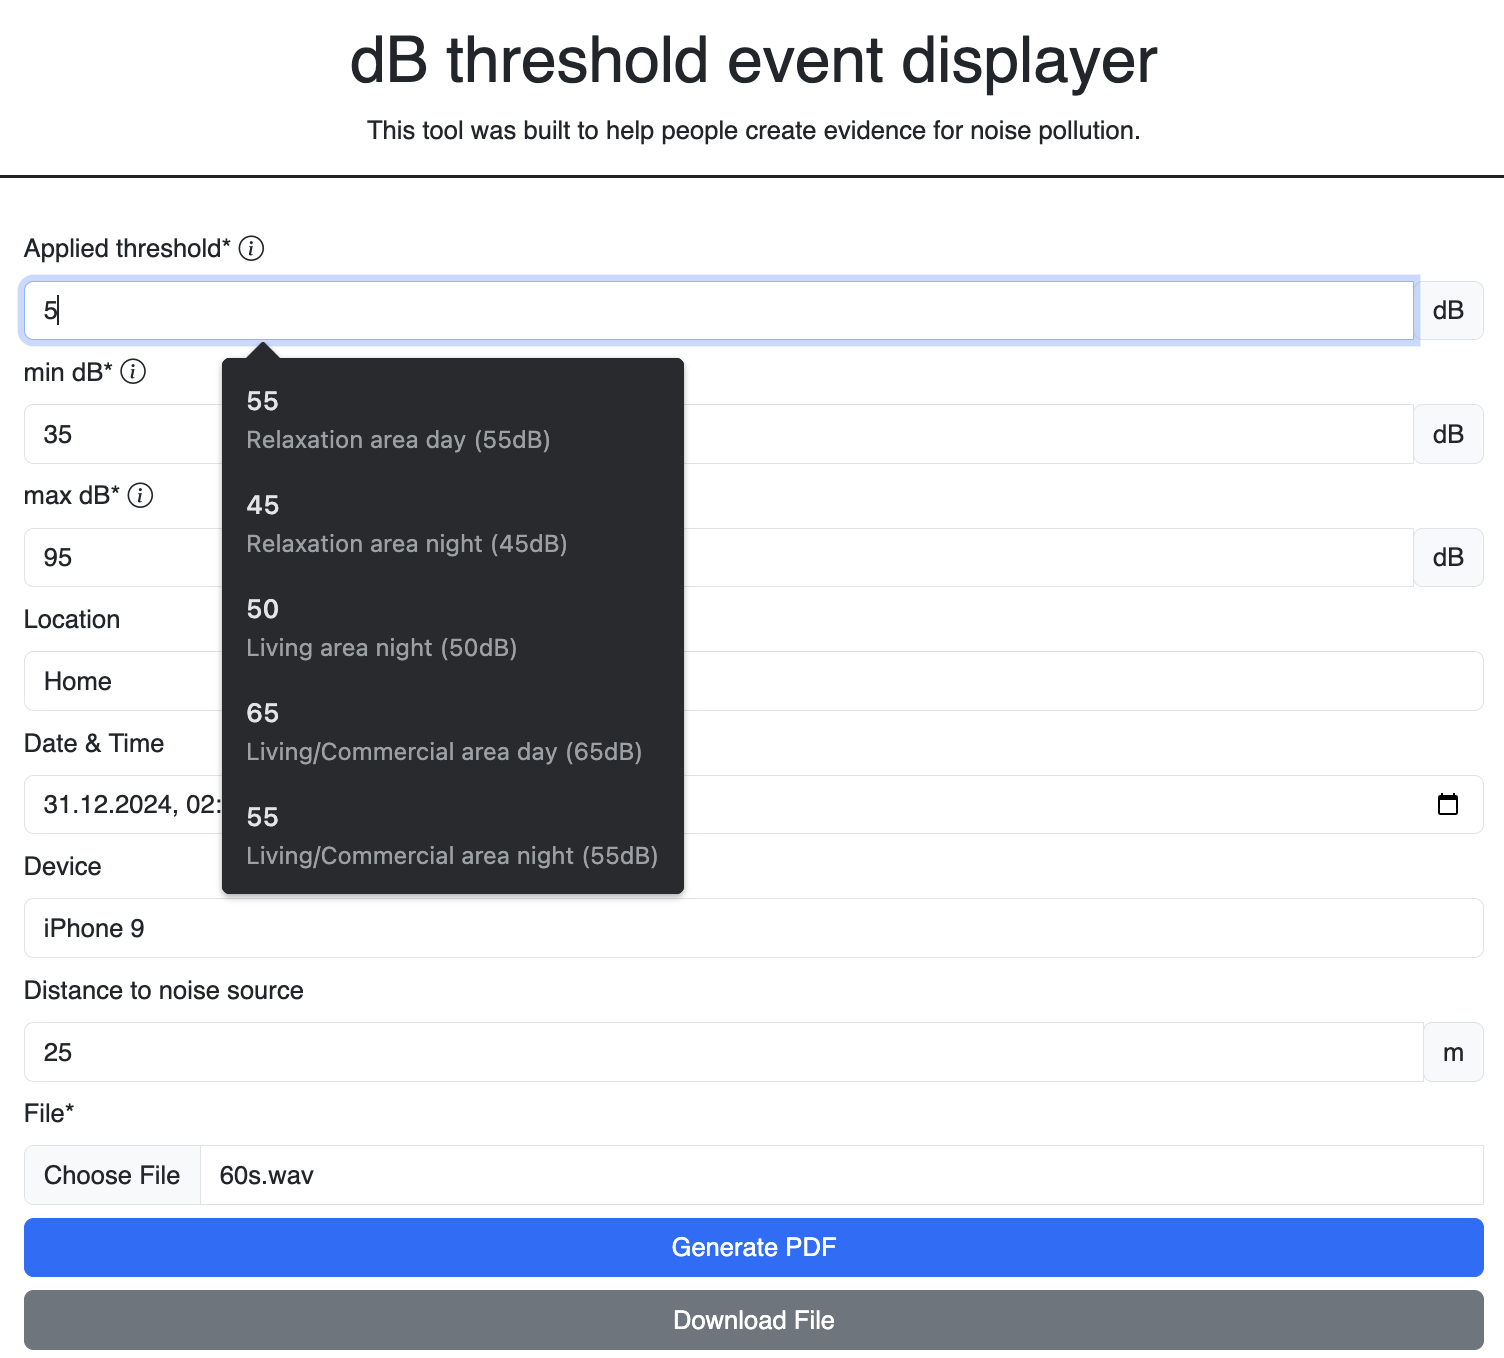
\includegraphics[width=0.475\textwidth]{../assets/abstract_application_screenshot.png}
%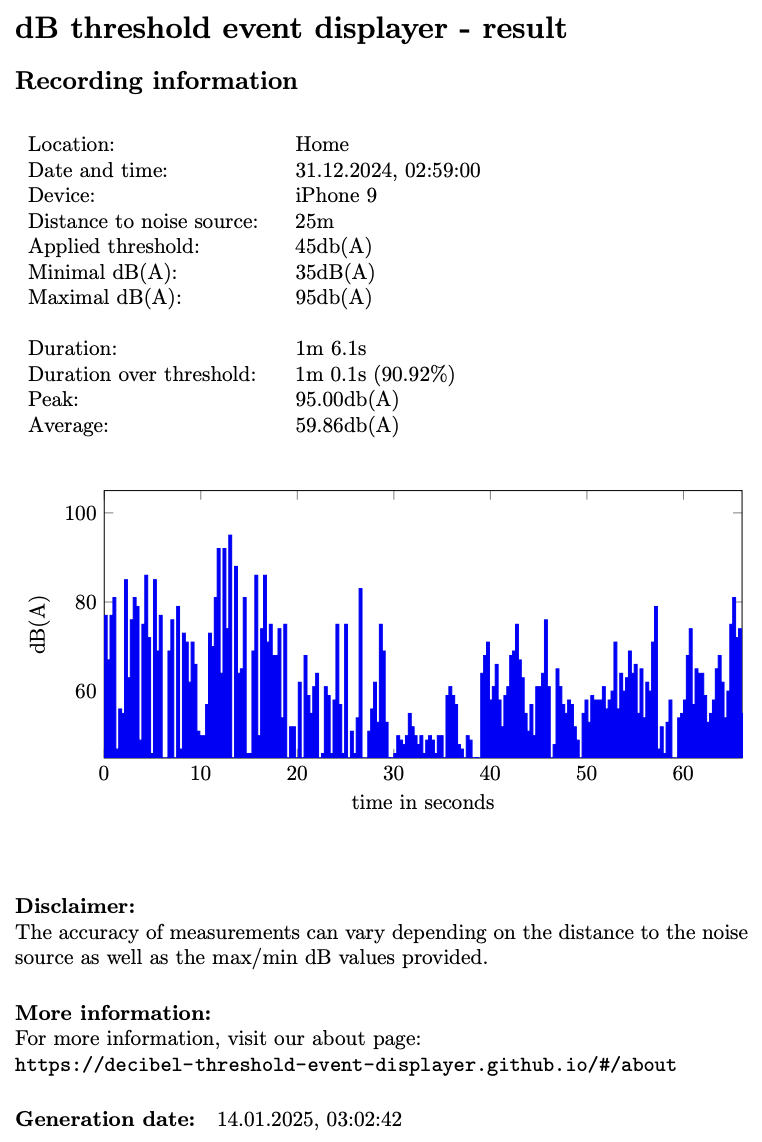
\includegraphics[width=0.475\textwidth]{../assets/abstract_report_screenshot.png}

\pagebreak
\end{abstract}
    \section{Table of contents}

\tableofcontents
    \section{List of Tables}

\begingroup
\hypersetup{hidelinks}
\listoftables
\endgroup
    \section{List of Figures}
\begingroup
\hypersetup{hidelinks}
\listoffigures
\endgroup
    \section{List of listings (code snipptes)}
Lorem ipsum

    \section{Introduction}\label{sec:introduction}

\subsection{Initial Situation}\label{subsec:initial-situation}
According to the~\href{https://www.bafu.admin.ch//}{Federal Office for the Environment} (DE:\ BAFU) one in seven people in Switzerland is affected by noise pollution~\cite{foen_noise_pollution}.
The pollution comes primarily from road traffic, followed by railways and then air traffic.
In addition to these noise sources, construction sites, nightclubs and public facilities also produce noise.
Because of this, Switzerland has set up upper noise limits that must be respected.
However, it is of course the case that these limits are not always adhered to.
Affected people must then either accept this or take action against it.
For the latter, they must gather evidence to prove their noise disturbance to the police and the courts.
This evidence then comes from an audio recording which the affected person made them self.

\subsection{Project Goal}\label{subsec:project-goal}
To help the people affected by noise pollution, we want to create an application which processes a given sound file (.wav)
and analyzes it.
It should detect when a specified threshold has been exceeded and then summarizes the result in a PDF document.
The document should then contain all necessary information for filing a complaint.
As our application will have a wide range of end users, two of our main design goals are to make it as user-friendly as possible
and to make it platform independent, so it can be used with any PC operating system and ideally mobile device.

\subsection{Problems with Audio Files}\label{subsec:problems-with-audio-files}
A wave file (.wav) contains samples of the recorded audio, where each sample represents the amplitude at a given moment.
Those amplitude values are relative to each other and not absolute.
It is therefore impossible to determine the actual dB(A) (loudness relative to the human ear) someone would perceive without any further information~\cite{adobe_community_how_to_know_the_real_world_db_level_of_a_file,stackoverflow_how_can_i_calculate_audio_db_level,stackexchange_exteracting_sound_pressure_from_wav_file}.
Because of this, we require the user to also give information about the minimal and maximal dB(A) measured in the given audio file.
To do this, we recommend using a smartphone app like \href{https://apps.apple.com/ch/app/dezibel-x-dba-l\%C3\%A4rm-messger\%C3\%A4t/id448155923}{DecibelX for IOS},
which allows the user to record the audio and also conveniently inspect the minimal and maximal dB measured in that recording.
With those two values, we can then map the relative values from the wave file to its db(A) values.
    \section{Specification}
The following chapter describes the system specification. The specification is derived from the requirements in the project description
as well as the discussions with the stakeholder. Assumptions and constraints are described in the following sections and were validated by
the defined product owner and the stakeholders if necessary.

\subsection{System Delimitation}
The system delimination is split into the static system environment (\ref{subsubsec:system_environment})
and the dynamic process environment (\ref{subsubsec:process_environment}).

\subsubsection{System Environment}
\label{subsubsec:system_environment}
System:
\begin{itemize}
    \item Frontend (User interaction)
    \item LaTeX and pgfplots
\end{itemize}
System context:
\begin{itemize}
    \item Stakeholder (tutor)
    \item User
    \item Lärmliga
    \item (Accurate conversion to absolute decibel)
\end{itemize}
Out of scope:
\begin{itemize}
    \item Integration in legal complaints
    \item (Accurate conversion to absolute decibel)
\end{itemize}

\subsubsection{Process Environment}
\label{subsubsec:process_environment}
\begin{itemize}
    \item Selecting a file
    \item WAV file analysis (validation, parsing, conversion to absolute db values, threshold filtering)
    \item Plotting (LaTeX / pgfplots) and PDF generation
\end{itemize}

\subsection{Requirements}
In the following section the requirements are detailed. Also the project boundaries and pre-conditions are described.

\subsubsection{Functional requirements}
The project team identified the following functional requirements:
\begin{table}[H]
    \centering
    \begin{tabularx}{\textwidth}{|c|X|c|c|c|}
        \hline
        \textbf{ID} & \textbf{Requirement} & \textbf{Priority} \\
        \hline
        R1 & Allow users to upload a .wav audio file. & MUST \\
        \hline
        R2 & Validate the uploaded file to ensure it is in .wav format, providing an error message if it is not. & MUST \\
        \hline
        R3 & Analyze the uploaded .wav file and calculate the noise level in decibels (dB). & MUST \\
        \hline
        R4 & Allow users to download the plotted noise data as an image or PDF. & MUST \\
        \hline
        R5 & Allow users to input metadata for the audio file, such as location, date, and time. & MUST \\
        \hline
        R6 & Plot the noise level data over time, with the x-axis representing time and the y-axis representing noise level (in dB). & MUST \\
        \hline
        R7 & Generate a PDF report including the plotted noise data and user input metadata. & MUST \\
        \hline
        R8 & Provide clear feedback and error messages. & SHOULD \\
        \hline
        R9 & Intuitive and responsive UI for selecting files, configuring options, and viewing results. & SHOULD \\
        \hline
        R10 & Allow the user to configure custom thresholds for noise levels. & COULD \\
        \hline
        R11 & Allow the user to change the language of the application. & COULD \\
        \hline
    \end{tabularx}
    \caption{Functional Requirements}
    \label{table:functional_requirements}
\end{table}

\subsubsection{Pre-Conditions and Boundaries}
Research done by the project team has revelead that reading absolute decibel values from WAV-files is more difficult than anticipated.
The reason for this is that normal consumer microphones are not calibrated for scientifically accurate measurements\cite{stackoverflow_spl}. Furthermore, it is trivial for a user
to increase the volume of a WAV-file using free, easy-to-use software like Audacity\cite{audacity}\cite{audacity_amplify}. Therefore, the project team has decided 
on a tentative working hypothesis together with the Stakeholder. \\ \\
Pre-Conditions:
\begin{itemize}
    \item The user must use a properly calibrated microphone or use a phone app which has built-in calibrations like Decibel X\cite{decibelx_ios}\cite{decibelx_android}.
    \item The user must have a way to export their audio recording as a WAV-file.
    \item The user must have access to a web browser capable of running WebAssembly.
    \item The user must not edit the exported WAV-file in any way except to decrease the length of the recording.
\end{itemize}
Boundaries:
\begin{itemize}
    \item The application supports only the analysis of pre-calibrated, un-edited WAV-files.
    \item The application supports only single-channel WAV-files.
    \item The user is presumed to be using properly calibrated equipment. There is no validation done in the application to ensure proper calibration.
    \item The user is presumed to be honest and to not have edited the WAV-file. There is no validation done in the application to ensure the file has not been edited.
\end{itemize}

\subsection{Usability}
Lorem ipsum

\subsubsection{Personas}
Lorem ipsum

\subsubsection{Storyboard}
Lorem ipsum

\subsubsection{UX-Prototyping}
Lorem ipsum
    \section{Evaluation}\label{sec:evaluation}

\subsection{Technology stack}\label{subsec:technology_stack}
Since the project description does not mention specific technologies to be used except for the LaTeX package pgfplots,
the project team decided to evaluate different technologies for the project by creating working prototypes.
The following chapters describe the evaluation criteria and the results of the evaluation.

\subsubsection{Criteria}
The following criteria are used to decide which technologies should be used for the project:
\begin{itemize}
    \item Know-how (10\%)
    \item Complexity (20\%)
    \item Usability (30\%)
    \item Distribution (40\%)
\end{itemize}

\subsubsection{Calculation}
The formula for calculating the weighted value of each criterion is:
\[
    v_w = \text{weight} \cdot \frac{\text{evaluation}}{5}
\]
Where \(evaluation\) is the scoring between 1--5.
The total score for a given technology is the sum
of weighted values.

\subsubsection{Technologies}
The following technologies were evaluated:
\begin{itemize}
    \item Kotlin with pdflatex as a dependency
    \item Kotlin bundled with pdflatex
    \item Website with SwiftLaTeX
\end{itemize}

\subsubsection{Reference LaTeX pgfplots template}\label{subsec:reference_latex_pgfplots_template}
For building the prototypes we will use the following reference LaTeX template which includes a pgfplots object:~\cite{pgfplots_gallery_sourceforge}

\begin{lstlisting}[caption={Reference LaTeX template with a pgfplots object},label={lst:reference_latex_pgfplots_template},language={[LaTeX]{TeX}}]
\documentclass{article}

\usepackage{siunitx}
\usepackage{tikz} % To generate the plot from csv
\usepackage{pgfplots}

\pgfplotsset{compat=newest} % Allows to place the legend below plot
\usepgfplotslibrary{units} % Allows to enter the units nicely

\sisetup{
  round-mode          = places,
  round-precision     = 2,
}

\begin{document}

\begin{figure}[h!]
  \begin{center}
    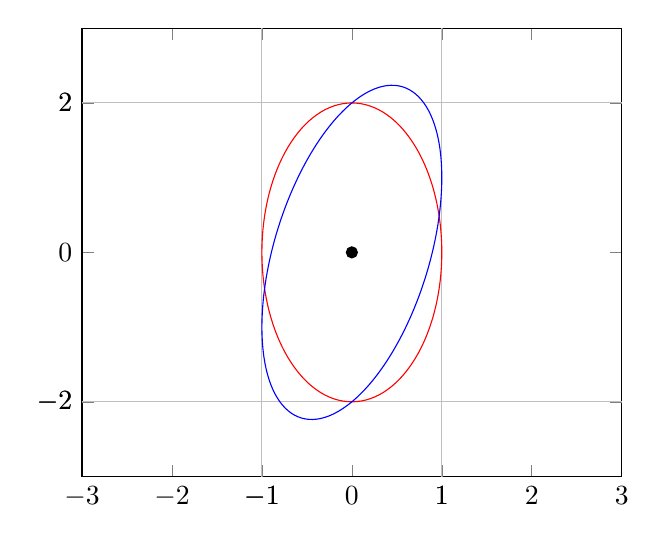
\begin{tikzpicture}
        \begin{axis}[
            xmin=-3,   xmax=3,
            ymin=-3,   ymax=3,
            extra x ticks={-1,1},
            extra y ticks={-2,2},
            extra tick style={grid=major},
        ]
            \draw[red] \pgfextra{
              \pgfpathellipse{\pgfplotspointaxisxy{0}{0}}
                {\pgfplotspointaxisdirectionxy{1}{0}}
                {\pgfplotspointaxisdirectionxy{0}{2}}
              % see also the documentation of
              % 'axis direction cs' which
              % allows a simpler way to draw this ellipse
            };
            \draw[blue] \pgfextra{
              \pgfpathellipse{\pgfplotspointaxisxy{0}{0}}
                {\pgfplotspointaxisdirectionxy{1}{1}}
                {\pgfplotspointaxisdirectionxy{0}{2}}
            };
            \addplot [only marks,mark=*] coordinates { (0,0) };
        \end{axis}
        \end{tikzpicture}
    \caption{My first autogenerated plot.}
  \end{center}
\end{figure}

\end{document}
\end{lstlisting}

\subsubsection{Kotlin minimal – Kotlin with pdflatex as a dependency}\label{subsubsec:kotlin_minimal}
This prototype uses Kotlin to satisfy platform-independence and invokes the pdflatex binary which is included in the TexLive distribution.
The project team chose to evaluate this technology because it satisfies the base requirements according to the project description and because
the project team is familiar with Kotlin.
Another advantage of this technology is that the distribution of the necessary LaTeX installation and packages is relegated to the user.
This greatly reduces distribution complexity.\newline
An obvious disadvantage of this approach is that the user needs to install TeXLive (and the pgfplots package) on their system, which might be difficult for non-technical users.

\paragraph{Licensing}\mbox{}\newline
This prototype is dependent on both TeXLive and pgfplots.
TeXLive uses a libre license that allows for the free redistribution with or without modifications~\cite{texlive_license} in accordance with the Free Software Foundation's free software definition~\cite{fsf_free_software}.
The pgfplots package uses the GPLv3 license~\cite{pgfplots}.

\paragraph{Evaluation}\mbox{}\newline
\begin{table}[H]
    \centering
    \begin{tabular}{l c c}
        \toprule
        \textbf{Criterion} & \textbf{Evaluation (1{-}5)} & \textbf{Weighted value} \\
        \midrule
        Know-how           & 4                           & 8                       \\
        \midrule
        Complexity         & 5                           & 20                      \\
        \midrule
        Usability          & 1                           & 6                       \\
        \midrule
        Distribution       & 5                           & 40                      \\
        \midrule
        \textbf{Total}     & n.a.                        & \textbf{74}             \\
        \bottomrule
    \end{tabular}
    \caption{Evaluation of Kotlin with pdflatex as a dependency}\label{table:kotlin_minimal_evaluation}
\end{table}

\subsubsection{Kotlin bundled – Kotlin bundled with pdflatex}\label{sec:kotlin_bundled}
Similarly to the prototype in~\fullref{subsubsec:kotlin_minimal}, this prototype uses Kotlin and invokes the pdflatex binary.
The major difference is that the pdflatex binary is provided alongside
the software.
The advantage of this approach is that the user does not have to install TexLive or any dependencies, greatly improving usability.
However, this comes with the disadvantage that the complexity of the distribution is much higher.
This approach also limits the advantages of using a platform-independent programming language because for every platform there has to be a release
which packages the appropriate binary.

\paragraph{Licensing}\mbox{}\newline
The licensing is equivalent to the licenses of the prototype in~\fullref{subsubsec:kotlin_minimal}.

\paragraph{Evaluation}\mbox{}\newline
\begin{table}[H]
    \centering
    \begin{tabular}{l c c}
        \toprule
        \textbf{Criterion} & \textbf{Evaluation (1{-}5)} & \textbf{Weighted value} \\
        \midrule
        Know-how           & 3                           & 6                       \\
        \midrule
        Complexity         & 3                           & 12                      \\
        \midrule
        Usability          & 5                           & 30                      \\
        \midrule
        Distribution       & 1                           & 8                       \\
        \midrule
        \textbf{Total}     & n.a.                        & \textbf{56}             \\
        \bottomrule
    \end{tabular}
    \caption{Evaluation of Kotlin bundled with pdflatex}\label{table:kotlin_bundled_evaluation}
\end{table}

\subsubsection{Web with SwiftLaTeX}
During the projects initial discussions, which had brainstorm like character, we wondered if we could render latex files directly in the browser, which would have the following benefits:
\begin{itemize}
    \item Providing the functionality as a web application would be probably the easiest and most accessible way for an end user to use the tool.
    \item Introducing the additional constraint of running the application only on the client side, would also avoid any infrastructure service and maintenance cost.
\end{itemize}
After a quick search we found the following open source JavaScript/WebWebassembly project: \href{https://www.swiftlatex.com/}{SwiftLaTeX: WYSIWYG LaTeX Editor for Browsers}
According to their website, the JavaScript/WebWebassembly library has the following characteristics~\cite{swiftlatex_website}:
\begin{itemize}
    \item 100\% Browser – PdfTeX and XeTeX written in WebAssembly and run in browsers.
    \item Compatibility – Produce exact same output you would get from TexLive or MikTeX\@.
    \item Library Support – Simply include a script tag and use PdfTeX or XeTeX in your own webpage.
    \item WYSIWYG – Support WYSIWYG editing on LaTeX documents using XeTeX engine.
    \item Speed – Run merely 2X slower than native binaries.
    \item Open Source – Completely Open Source. You can find the code on \href{https://github.com/SwiftLaTeX/SwiftLaTeX/}{GitHub}.
\end{itemize}
If the statements on the SwiftLaTeX website hold true, it would neatly full-fill our requirements for building a client side only web application.

\paragraph{Verifying basic functionality}\mbox{}\newline
To make a first feasibility test we can insert our reference LaTeX pgfplots template~\autoref{lst:reference_latex_pgfplots_template} into the \href{https://www.SwiftLaTeX.com/\#demo}{SwiftLaTeX Demo tool}.
Even though it took more than one and a half minute to process, we were very surprised that this just worked, see figure~\autoref{fig:SwiftLaTeX_demo_rendering_latex_pgfplots_template}:
\begin{figure}[H]
    \centering
    \includegraphics[width=0.5\textwidth]{SwiftLaTeX_demo_pgfplots}
    \caption{Screenshot of the SwiftLaTeX Demo tool rendering the reference LaTeX pgfplots template}\label{fig:SwiftLaTeX_demo_rendering_latex_pgfplots_template}
\end{figure}

\paragraph{Investigating dependencies are loaded}\mbox{}\newline
After investigating what actually happens on the page with the browsers developer tools network tab, we saw that SwiftLaTeX will load all dependencies asynchronously via https://texlive2.SwiftLaTeX.com/.
This process and how self-host those files, is documented in the README.md of the SwiftLaTeX GitHub library~\cite{SwiftLaTeX_github_repository}.
As we will be able to specify which LaTeX dependencies our application will use, it would be interesting to download and serve only the files we actually need.
We also saw that the dependencies are loaded sequentially, which we would like to optimize to reduce the pdf generation time.

\paragraph{Local development setup}\mbox{}\newline
To make the same example working on a local machine, we can download the latest release from the GitHub repository: \href{https://github.com/SwiftLaTeX/SwiftLaTeX/releases/tag/v20022022}{Releases 20/02/2022}.
The release contains the website visible at \href{https://www.SwiftLaTeX.com/}{SwiftLaTeX.com} including the compiled WebAssembly files.
As expected, opening the index.html file from the unzipped release folder in a browser will look like the website \href{https://www.SwiftLaTeX.com/}{SwiftLaTeX.com}.
Validating the basic functionality with our reference LaTeX pgfplots template~\autoref{lst:reference_latex_pgfplots_template} did not work, as we get the following error message in the JavaScript console:
\begin{lstlisting}[caption={SwiftLaTeX local development setup: JavaScript error message},label={lst:SwiftLaTeX_local_setup_js_error}]
PdfTeXEngine.js:89 Uncaught (in promise) SecurityError: Failed to construct 'Worker': Script at 'file:///home/lukas/Downloads/20-02-2022/SwiftLaTeXpdftex.js' cannot be accessed from origin 'null'.
...
\end{lstlisting}

According to the following \href{https://stackoverflow.com/questions/21408510/chrome-cant-load-web-worker}{stackoverflow question}, Google Chrome does not load web workers when running scripts from local files.
The web worker is required to run WebAssembly, which does all the actual LaTeX to PDF transformation in this prototype.
The easiest solution for this issue is to run a webserver, luckily this is trivial with Python.
We just have to run the following command in the directory of the unpacked SwiftLaTeX release folder:
\begin{lstlisting}[caption={Start a webserver on http://localhost:8000/ with Python},language=bash,label={lst:lstlisting}]
python -m http.server
\end{lstlisting}
Validating the basic functionality with our reference LaTeX pgfplots template~\autoref{lst:reference_latex_pgfplots_template} on http://localhost:8000/ works now as expected.

\paragraph{Distribution option 1: Python webserver}\mbox{}\newline
This would be the easiest solution, as it is analog to the local development setup described in the previous paragraph.
But installing Python, downloading the git repository or downloading a release and running the Python web server in the correct directory, requires at least a lot of technical affinity.

\paragraph{Distribution option 2: PyInstaller}\mbox{}\newline
To enhance the end users experience we could build an executable from a Python file with PyInstaller which supports builds for Windows, macOS and Linux.
Even though this solution worked in a quick proof of concept on a linux system, the user would need to find the public GitLab repository and download a release, which contains the latest executables.
Further the user might have security concerns, as downloading an executable from an unknown or untrusted source is really dangerous.

\paragraph{Distribution option 3: GitHub Pages}\mbox{}\newline
After thinking about it, we figured out that we could deploy the tool as a static HTML page to GitHub pages, this would resolve the need of downloading any source code or executable program.
In our opinion this would result in the best user experience, as the user only needs a web browser to access and use the tool.
As this solution was worth exploring, we deployed the prototype with GitHub pages: https://vonal3.github.io/

\paragraph{Licensing}
\begin{itemize}
    \item SwiftLaTeX:\ \href{https://github.com/SwiftLaTeX/SwiftLaTeX/blob/master/LICENSE}{SwiftLaTeX License}, \href{https://www.gnu.org/licenses/agpl-3.0.en.html}{GNU AFFERO GENERAL PUBLIC LICENSE}
    \item LaTeX:\ \href{https://www.latex-project.org/lppl.txt}{The LaTeX project public license}
    \item TeXLive:\ \href{https://www.tug.org/texlive/copying.html}{TeX Live licensing, copying, and redistribution}, \href{https://www.tug.org/texlive/LICENSE.TL}{COPYING CONDITIONS FOR TeX Live}
    \item pgfplots:\ \href{https://ctan.org/pkg/pgfplots}{https://ctan.org/pkg/pgfplots}, \href{https://www.gnu.org/licenses/gpl-3.0.en.html}{GNU General Public License, version 3 or newer}
\end{itemize}

\paragraph{Evaluation}\mbox{}\newline
\begin{table}[H]
    \centering
    \begin{tabular}{l c c}
        \toprule
        \textbf{Criterion} & \textbf{Evaluation (1{-}5)} & \textbf{Weighted value} \\
        \midrule
        Know-how           & 3                           & 6                       \\
        \midrule
        Complexity         & 3                           & 12                      \\
        \midrule
        Usability          & 4                           & 24                      \\
        \midrule
        Distribution       & 5                           & 40                      \\
        \midrule
        \textbf{Total}     & n.a.                        & \textbf{82}             \\
        \bottomrule
    \end{tabular}
    \caption{Evaluation of SwiftLaTeX JavaScript/WebAssembly library}\label{table:SwiftLaTeX_evaluation}
\end{table}

\subsubsection{Chosen Solution}
Using the evaluations given to the selected technologies, the following demonstrates the combined results:
\begin{table}[H]
    \centering
    \begin{tabular}{l c c}
        \toprule
        \textbf{Technology} & \textbf{Total score} \\
        \midrule
        Kotlin minimal      & 74                   \\
        \midrule
        Kotlin bundled      & 56                   \\
        \midrule
        Web SwiftLaTeX      & 82                   \\
        \bottomrule
    \end{tabular}
    \caption{Technology stack evaluation}\label{table:technology_evaluation}
\end{table}
In accordance with the table above, the project team decided to use \textbf{Web SwiftLaTeX} with the distribution option 3 \textbf{GitHub Pages}.

\subsection{License}\label{subsec:evaluation-license}
After evaluating the different possible technologies, the following third party software will be used:
\begin{itemize}
    \item SwiftLaTeX: \href{https://github.com/SwiftLaTeX/SwiftLaTeX/blob/master/LICENSE}{SwiftLaTeX License}, \href{https://www.gnu.org/licenses/agpl-3.0.en.html}{GNU AFFERO GENERAL PUBLIC LICENSE}
    \item LaTeX: \href{https://www.latex-project.org/lppl.txt}{The LaTeX project public license} (GPL Compatible)
    \item TeXLive: \href{https://www.tug.org/texlive/copying.html}{TeX Live licensing, copying, and redistribution}, \href{https://www.tug.org/texlive/LICENSE.TL}{COPYING CONDITIONS FOR TeX Live} (GPL Compatible)
    \item pgfplots: \href{https://ctan.org/pkg/pgfplots}{https://ctan.org/pkg/pgfplots}, \href{https://www.gnu.org/licenses/gpl-3.0.en.html}{GNU General Public License, version 3 or newer}
    \item Bootstrap: \href{https://github.com/twbs/bootstrap/blob/main/LICENSE}{Bootstrap License}, \href{https://en.wikipedia.org/wiki/MIT_License}{MIT License} (GPL Compatible)
\end{itemize}
To be conform with the used software, we will also publish our code under the \href{https://www.gnu.org/licenses/gpl-3.0.en.html}{GPL-3.0 licence (FLOSS)}.

    \section{Implementation}
Lorem ipsum

\subsection{Architecture}
Lorem ipsum

\subsection{Processes}
Lorem ipsum


    \section{Deployment and Integration}\label{sec:deployment-and-integration}
We decided to use GitHub Pages via an \href{https://github.com/decibel-threshold-event-displayer}{organization} for distribution because it provides an easy way to access the
application for end users and simplifies the maintenance for developers. The application is then available as a \href{https://decibel-threshold-event-displayer.github.io/}{Github Page}.
The following list and the graphic~\autoref{fig:deployment_flow} elaborates on the deployment workflow.

\begin{enumerate}
    \item A dev pushes or merges code to the main branch
    \item GitLab automatically mirrors the repository to GitHub
    \item GitHub deploys automatically to GitHub Pages
    \item {The Application is available under: \\
          \href{https://decibel-threshold-event-displayer.github.io/}{https://decibel-threshold-event-displayer.github.io/}}
\end{enumerate}

\begin{figure}[H]
    \centering
    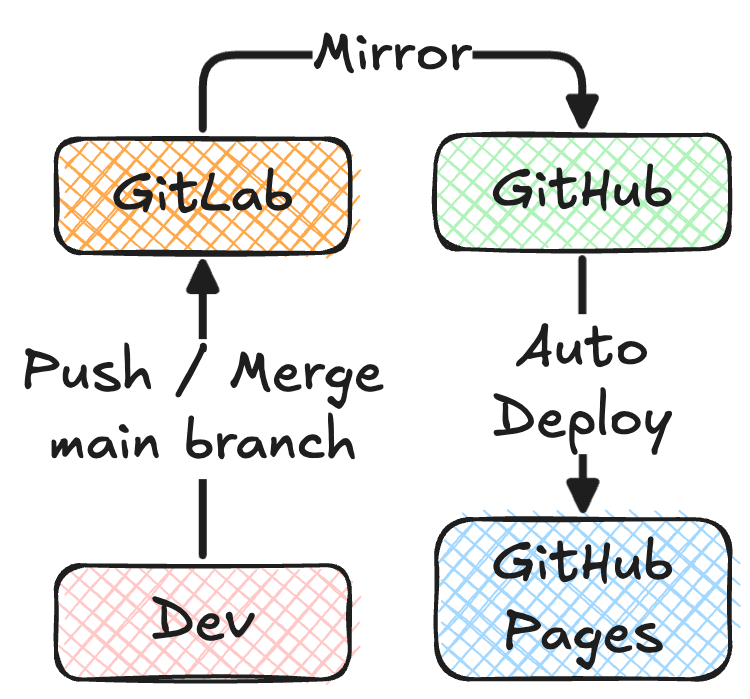
\includegraphics[width=0.5\textwidth]{../assets/deployment_and_distribution.png}
    \caption{Deployment Flow}\label{fig:deployment_flow}
\end{figure}

\subsection{Installation Manual \& Script}\label{subsec:installation-manuel-and-script}
We are using a Makefile to automate the development setup, build and deploy the application to GitHub Pages.

\subsubsection{Development setup}\label{subsubsec:deployment-setup}
A local webserver is needed work on the application as some Browsers will not execute web workers on locally served files~\cite{stackoverflow_chrome_cant_load_web_worker}.
By default, the project uses the built-in webserver of Python 3.
Python 3 can be installed with the systems package manager or by downloading it from the \href{https://www.python.org/downloads/}{official website}.
Afterward the following command can be used to run the local webserver on \href{http://0.0.0.0:8000/}{0.0.0.0:8000/\#/}:

\begin{lstlisting}[caption={Makefile: Start local webserver},label={lst:makefile_start_local_webserver},language=Bash]
$ make dev
\end{lstlisting}

\subsubsection{Distribution}
The project and the repository is managed via the GitLab of BFH,
but we want to use GitHub pages to deploy and distribute our application,
the project team decided that we mirror the GitLab repository to GitHub:
\begin{itemize}
    \item \href{https://gitlab.ti.bfh.ch/decibel-threshold-event-displayer/decibel-threshold-event-displayer}{GitLab Repository}
    \item \href{https://github.com/decibel-threshold-event-displayer/decibel-threshold-event-displayer.github.io}{GitHub Repository}
\end{itemize}

\paragraph{Mirror setup:}
\begin{enumerate}
    \item Log into \href{https://gitlab.ti.bfh.ch}{gitlab.ti.bfh.ch}
    \item Navigate to the repository: \href{https://gitlab.ti.bfh.ch/decibel-threshold-event-displayer/decibel-threshold-event-displayer/}{GitLab Repository}
    \item Go to the repositories settings page: \href{https://gitlab.ti.bfh.ch/decibel-threshold-event-displayer/decibel-threshold-event-displayer/-/settings/repository}{Settings > Repository}
    \item Open the Tab ``Mirroring repositories``
    \item Click the button ``Add new``
    \item Fill the form as follows:
          \begin{itemize}
              \item Git repository URL: ssh://git@github.com/decibel-threshold-event-displayer/decibel-threshold-event-displayer.github.io.git
              \item Mirror direction: Pull
              \item Authentication method: SSH public key
              \item Username: github
              \item Mirror user: autofilled
              \item Overwrite diverged branches: Select
              \item Mirror branches > Mirror specific branches: main
          \end{itemize}
    \item Click the button ``Mirror repository``
    \item The first try will fail, as we have to add the public key generated by GitLab to the GitHub repository
    \item On the newly created entry, click the clipboard button ``Copy SSH public key`` (the public key is now in your clipboard)
    \item Keep the current GitLab tab open
    \item Log into \href{https://github.com/}{github.io} in a new tab
    \item Navigate to the repository: \href{https://github.com/decibel-threshold-event-displayer/decibel-threshold-event-displayer.github.io/}{GitHub Repository}
    \item Go to the repositories deploy keys page: \href{https://github.com/decibel-threshold-event-displayer/decibel-threshold-event-displayer.github.io/settings/keys}{Settings > Deploy Keys}
    \item Click the button ``Add deploy key``
    \item Fill the form as follows:
          \begin{itemize}
              \item Title: github
              \item Key: Copy the SSH public key from the clipboard
              \item Allow write access: yes
          \end{itemize}
    \item Click the button ``Add Key``
    \item Go back to the gitlab tab
    \item Click the reload button ``Update now``
    \item Wait until the process is finished
\end{enumerate}

\subsubsection{Build}
As we have only plain JavaScript files, we don't have a build step.

\subsubsection{Deploy}
As described above, we created a Mirror of this repository on GitHub.
Based on the following documentation, we configured GitHub to automatically deploy to GitHub Pages:
\href{https://docs.github.com/en/pages/getting-started-with-github-pages/creating-a-github-pages-site}{Creating a GitHub Pages site}

Further we had to add a configuration file under ``.github/workflows/static.yml`` and change value of \texttt{path: './'} to \texttt{path: './app'}.
The initial file was generated by the following setup page:
\href{https://github.com/decibel-threshold-event-displayer/decibel-threshold-event-displayer.github.io/new/main?filename=.github%2Fworkflows%2Fstatic.yml&pages_workflow_template=pages%2Fstatic}{Repository > Settings > GitHub Pages > Static HTML > Configure}

\subsection{User Manual}\label{subsec:user-manuel}
The project team decided to not create an additional document for the user manual,
because all the necessary information for using the application are provided by following list of best practices:
\begin{itemize}
    \item Following common UI patterns
    \item Well-known form components
    \item Tooltips where needed
    \item Human-readable error messages
    \item About page with detailed technical information
\end{itemize}


    \begin{frame}
    \frametitle{Conclusion}
\end{frame}
    \section{Glossary}


    \section{Index}
Lorem ipsum


    \section{Bibliography}
Lorem ipsum

    \section{Appendix}\label{sec:appendix}

\subsection{Project description}\label{subsec:project-description}

The \textbf{goal (what)} of this project is to deliver a FLOSS-licensed, platform-independent piece of
software (computer program), called the \textit{Decibel Threshold Event Displayer}, that

\begin{enumerate}
    \item takes as inputs a WAV-file and a list of sound level thresholds in decibels (e.g., legal day
          and nighttime noise maxima above which your health deteriorates);
    \item filters out all data points in the file that correspond to sound events below the lowest of
          the above thresholds; and
    \item displays the remaining data points (as a blue vertical comb plot) on a horizontal time
          axis (with the dates and times corresponding to the data points) as well as the
          thresholds (as horizontal red lines) in decibel, and statistically summarises the data set
          with the help of the LaTeX-package pgfplots.
\end{enumerate}

The \textbf{purpose (why)} of this project is to empower poor folks who suffer from insomnia due to
ambient noise (\url{https://laermliga.ch/}) by arming them with the (peaceful) means of proving
their noise hell (a smartphone app such as \url{https://apps.apple.com/ch/app/dezibel-x-pro-l\%C3\%A4rm-messger\%C3\%A4t/id1257651611}
together with your software) to the police and the courts of law. \\

The code should be minimal, modular, and self-explaining. \\

The project report should be concise (maximally informative, minimally long). It must contain
this project description as a quotation.

\subsection{Declaration of Authorship}\label{subsec:declaration-of-authorship}
The project team, namely Dominic Gernert, Lukas von Allmen, and Darius Degel, hereby declare that the report submitted is our own unaided work.
All direct or indirect sources used are acknowledged as references.
\end{document}
